% ─────────────────────────────────────────────────────────────────────────────
% chapters/ch2_analysis.tex — Chapter 2: Requirements Analysis and System Design
% ─────────────────────────────────────────────────────────────────────────────

\chapter{Requirements Analysis and System Design}

Building on the state of the art surveyed in Chapter~1, this chapter formalises the requirements of \textit{Mobile Match Algeria} and presents the architectural and design decisions taken to meet them. The chapter covers requirements gathering, actor identification, UML modelling, data model definition, system architecture, UI/UX principles, and technology stack justification.

\section{Requirements Gathering}

\subsection{Methodology}

Requirements were elicited through two complementary methods. First, the three operator websites (Mobilis, Djezzy, Ooredoo) were systematically examined to identify the information currently available to consumers and the limitations of each operator's self-presentation. Second, the international comparison platforms reviewed in Chapter~1 were analysed to extract implicit requirements from observed best practices and identified gaps. This dual approach grounded the requirement set in both the specific constraints of the Algerian market and the established conventions of the broader plan-comparison domain.

\subsection{Functional Requirements}

Table~\ref{tab:fr} lists the nine functional requirements elicited, ordered by priority.

\begin{table}[H]
  \caption{Functional requirements}
  \label{tab:fr}
  \centering\small
  \begin{tabular}{|p{1.2cm}|p{9.5cm}|p{3.2cm}|}
    \hline
    \textbf{ID} & \textbf{Description} & \textbf{Actor} \\
    \hline
    FR1 & Display all current mobile plans from Mobilis, Djezzy, and Ooredoo with their key attributes: price, data volume, voice minutes, SMS allowance, validity period, and network generation. & All users \\
    \hline
    FR2 & Filter the plan catalogue by operator, plan type (prepaid, postpaid, data-only), maximum price, minimum data volume, and network generation. & All users \\
    \hline
    FR3 & Select up to three plans and view them in a side-by-side comparison table with best-value highlighting per attribute row. & All users \\
    \hline
    FR4 & Define a usage profile (budget, data, voice, SMS, preferred type, preferred network) and receive a ranked list of the three best-matching plans produced by the scoring engine. & Registered User \\
    \hline
    FR5 & Bookmark any plan from the offers page, access all bookmarked plans from a dedicated saved-plans page, and remove individual bookmarks. & Registered User \\
    \hline
    FR6 & Receive in-app notifications when new plans are added to the catalogue; mark individual or all notifications as read; delete individual notifications. & Registered User \\
    \hline
    FR7 & Automatically scrape offer data from the three operator websites on a daily schedule and update the database with new, changed, and deactivated plans. & System \\
    \hline
    FR8 & Trigger manual scrape runs, view detailed per-operator scrape logs, monitor platform statistics, and manage system notifications from the admin dashboard. & Administrator \\
    \hline
    FR9 & Register a new account, log in with email and password, and log out. Passwords must be stored using a one-way hashing algorithm. & All users \\
    \hline
  \end{tabular}
\end{table}

\subsection{Non-Functional Requirements}

Table~\ref{tab:nfr} lists the five non-functional requirements that constrain the system's quality attributes.

\begin{table}[H]
  \caption{Non-functional requirements}
  \label{tab:nfr}
  \centering\small
  \begin{tabular}{|p{1.3cm}|p{2.8cm}|p{9.9cm}|}
    \hline
    \textbf{ID} & \textbf{Category} & \textbf{Constraint} \\
    \hline
    NFR1 & Performance    & Page load time for the offers listing must not exceed 2~seconds on a standard broadband connection. \\
    \hline
    NFR2 & Responsiveness & The interface must be fully usable on mobile devices (320~px viewport and above), tablets, and desktop screens. \\
    \hline
    NFR3 & Security       & User sessions must be managed with signed JWT tokens; passwords must be hashed with bcrypt; all admin-only routes must verify the user role before processing the request. \\
    \hline
    NFR4 & Maintainability & The codebase must be organised into clearly separated modules (scrapers, recommendation engine, API routes, UI components) to facilitate future extension and maintenance. \\
    \hline
    NFR5 & Accuracy       & Scraped offer data must be normalised against a common schema; any discrepancy or scraping error must be recorded in the ScrapeLog for operator monitoring. \\
    \hline
  \end{tabular}
\end{table}

\section{System Actors}

Three actor types interact with the system, as summarised in Table~\ref{tab:actors}.

\begin{table}[H]
  \caption{System actors and their capabilities}
  \label{tab:actors}
  \centering\small
  \begin{tabular}{|p{3.5cm}|p{11.5cm}|}
    \hline
    \textbf{Actor}  & \textbf{Capabilities} \\
    \hline
    Visitor         & Browse offers, apply filters, view offer details, compare up to 3 plans \\
    \hline
    Registered User & All visitor capabilities + save plans, view saved plans, receive notifications, set usage profile, get personalised recommendations \\
    \hline
    Administrator   & All user capabilities + trigger scrape runs, view scrape logs, monitor platform statistics, manage notifications \\
    \hline
  \end{tabular}
\end{table}

\section{UML Use Case Diagrams}

The main use cases of the system are organised around three actors. Figure~\ref{fig:usecase-main} illustrates the top-level use case diagram.

\begin{figure}[H]
\centering
\begin{tikzpicture}[
  actor/.style={rectangle, draw=black!60, fill=gray!10, rounded corners=3pt,
                minimum width=2.4cm, minimum height=0.65cm, align=center, font=\small\bfseries},
  uc/.style={ellipse, draw=black!70, fill=blue!6, minimum width=4.0cm, minimum height=0.75cm,
             align=center, font=\small},
  ucadm/.style={ellipse, draw=black!70, fill=orange!10, minimum width=4.0cm, minimum height=0.75cm,
                align=center, font=\small},
  sys/.style={rectangle, draw=black!50, dashed, rounded corners=5pt, inner sep=10pt},
  assoc/.style={thick, black!55},
  gen/.style={thick, black!70, -{Triangle[open, length=6pt, width=6pt]}}
]
  % System boundary (all actors on the LEFT, use cases on the RIGHT)
  \node[sys, minimum width=9cm, minimum height=10.2cm] (sys) at (6.5,-4.5) {};
  \node[font=\small\bfseries, anchor=north west] at (sys.north west) {\textit{Mobile Match Algeria}};

  % Use cases
  \node[uc]    (uc1) at (6.5,-0.8) {Browse \& Filter Offers};
  \node[uc]    (uc2) at (6.5,-2.1) {Compare Plans (side-by-side)};
  \node[uc]    (uc3) at (6.5,-3.4) {Get Recommendations};
  \node[uc]    (uc4) at (6.5,-4.7) {Save \& Manage Plans};
  \node[uc]    (uc5) at (6.5,-6.0) {Edit Usage Profile};
  \node[ucadm] (uc6) at (6.5,-7.4) {Trigger Scrape Run};
  \node[ucadm] (uc7) at (6.5,-8.6) {View Scrape Logs \& History};

  % Actors — all on the LEFT in a vertical column
  \node[actor] (visitor) at (0.2,-1.45) {Visitor};
  \node[actor] (user)    at (0.2,-4.7)  {Registered\\User};
  \node[actor] (admin)   at (0.2,-8.0)  {Administrator};

  % Generalisation arrows (open triangle = is-a; no label)
  \draw[gen] (user.north)  -- (visitor.south);
  \draw[gen] (admin.north) -- (user.south);

  % Visitor associations
  \draw[assoc] (visitor.east) -- (uc1.west);
  \draw[assoc] (visitor.east) -- (uc2.west);

  % Registered User associations
  \draw[assoc] (user.east) -- (uc3.west);
  \draw[assoc] (user.east) -- (uc4.west);
  \draw[assoc] (user.east) -- (uc5.west);

  % Administrator associations
  \draw[assoc] (admin.east) -- (uc6.west);
  \draw[assoc] (admin.east) -- (uc7.west);
\end{tikzpicture}
\caption{Top-level use case diagram for Mobile Match Algeria}
\label{fig:usecase-main}
\end{figure}

Table~\ref{tab:usecases} describes each primary use case, the actor who triggers it, and its behaviour.

\begin{table}[H]
  \caption{Primary use cases of Mobile Match Algeria}
  \label{tab:usecases}
  \centering\small
  \begin{tabular}{|p{1.1cm}|p{3.8cm}|p{2.8cm}|p{6.0cm}|}
    \hline
    \textbf{ID} & \textbf{Use Case} & \textbf{Actor(s)} & \textbf{Description} \\
    \hline
    UC1 & Browse \& Filter Offers    & All users         & Access the offers page and apply any combination of filters (operator, type, price, data, network); the system retrieves matching plans and renders them as interactive cards. \\
    \hline
    UC2 & Compare Plans              & All users         & Select up to three plans and view them in a side-by-side table with best-value highlighting per attribute row. Requires at least two plans selected. \\
    \hline
    UC3 & Get Recommendations        & Registered User   & Submit a usage profile and receive a ranked list of the three best-matching plans produced by the scoring engine, with a score breakdown for each result. \\
    \hline
    UC4 & Save \& Manage Plans       & Registered User   & Bookmark any plan from the offers page, access all saved plans from a dedicated page, compare them, or remove individual bookmarks. \\
    \hline
    UC5 & Edit Usage Profile         & Registered User   & Update usage preferences (budget, data volume, voice minutes, SMS allowance, plan type, network) from the profile page. The updated profile is applied the next time UC3 is invoked. \\
    \hline
    UC6 & Trigger Scrape Run         & Administrator     & Initiate a scrape run for one or all operators from the admin dashboard; the system updates the catalogue, creates notifications for new offers, and records a ScrapeLog entry. \\
    \hline
    UC7 & View Scrape Logs \& History & Administrator    & Consult the full scrape history log, inspect per-operator event lines (offers found, inserted, updated, errors), and assess pipeline health to detect failures and evaluate catalogue freshness. \\
    \hline
  \end{tabular}
\end{table}

\section{UML Activity and Sequence Diagrams}

\subsection{Scraping Pipeline Activity Diagram}

Figure~\ref{fig:activity-scrape} represents the activity flow of the automated scraping pipeline, from trigger to database update.

\begin{figure}[H]
\centering
\begin{tikzpicture}[
  node distance=0.55cm and 1.2cm,
  startstop/.style={ellipse, draw, fill=gray!20, minimum width=2.8cm, minimum height=0.7cm, font=\small\bfseries},
  process/.style={rectangle, rounded corners=3pt, draw, fill=blue!8, minimum width=5.5cm, minimum height=0.7cm, align=center, font=\small},
  decision/.style={diamond, draw, fill=orange!15, aspect=2.8, minimum height=0.7cm, align=center, font=\small},
  arrow/.style={-{Stealth[length=5pt]}, thick}
]
  \node[startstop] (start) {START};
  \node[process, below=of start] (trigger) {Cron trigger or Admin action};
  \node[process, below=of trigger] (fetch) {Fetch operator page (HTTP GET)};
  \node[process, below=of fetch] (parse) {Parse HTML / DOM, extract raw offers};
  \node[process, below=of parse] (norm) {Normalise data (units, slugs, types)};
  \node[decision, below=of norm] (exists) {Offer already\\in DB?};
  \node[process, right=1.8cm of exists] (update) {UPDATE record};
  \node[process, below=0.9cm of exists] (insert) {INSERT new offer \& notify users};
  \node[process, below=0.6cm of insert] (deact) {Deactivate offers absent from scrape\\(partial-scrape guard applied)};
  \node[process, below=of deact] (log) {Write ScrapeLog (status, counts, duration)};
  \node[startstop, below=of log] (end) {END};

  \draw[arrow] (start) -- (trigger);
  \draw[arrow] (trigger) -- (fetch);
  \draw[arrow] (fetch) -- (parse);
  \draw[arrow] (parse) -- (norm);
  \draw[arrow] (norm) -- (exists);
  \draw[arrow] (exists) -- node[above, font=\scriptsize]{Yes} (update);
  \draw[arrow] (update) |- (deact);
  \draw[arrow] (exists) -- node[right, font=\scriptsize]{No} (insert);
  \draw[arrow] (insert) -- (deact);
  \draw[arrow] (deact) -- (log);
  \draw[arrow] (log) -- (end);
\end{tikzpicture}
\caption{Activity diagram --- automated scraping pipeline}
\label{fig:activity-scrape}
\end{figure}

The pipeline begins when a cron trigger or administrator action initiates a scrape for a given operator. The scraper fetches the operator's plan page, parses and normalises the data, and compares each scraped offer against the existing database entries. New offers are inserted; existing offers with changed attributes are updated; offers absent from the scraped data are marked inactive. A ScrapeLog record is created regardless of outcome, recording the number of offers found, inserted, updated, and any error encountered.

\subsection{Recommendation Request Sequence Diagram}

Figure~\ref{fig:seq-recommend} illustrates the sequence of interactions between the client, the API server, the database, and the recommendation engine when a registered user requests personalised recommendations.

\begin{figure}[H]
\centering
\begin{tikzpicture}[
  actor/.style={rectangle, draw=black!70, fill=gray!15, minimum width=2.8cm,
                minimum height=0.55cm, align=center, font=\small\bfseries},
  msg/.style={-{Stealth[length=4pt]}, thick},
  retmsg/.style={-{Stealth[length=4pt]}, thick, dashed},
  note/.style={font=\scriptsize, fill=yellow!20, draw=gray!60,
               rounded corners=2pt, inner sep=3pt, align=left}
]
  % Participants — 4.0 cm apart
  \node[actor] (client) at (0,0)    {Client Browser};
  \node[actor] (api)    at (4.0,0)  {API Server};
  \node[actor] (db)     at (8.0,0)  {Database};
  \node[actor] (engine) at (12.0,0) {Rec.\ Engine};

  % Lifelines
  \foreach \x in {0,4.0,8.0,12.0}
    \draw[gray!50, thick] (\x,-0.35) -- (\x,-7.8);

  % 1. POST request
  \draw[msg] (0,-0.9) -- (4.0,-0.9)
    node[midway, above, font=\scriptsize]{POST /api/recommendations \{profile\}};

  % 2. API-internal: validate (node, not zero-length arrow)
  \node[note, anchor=west] at (4.3,-1.7) {Validate JWT session};

  % 3. Fetch active offers
  \draw[msg] (4.0,-2.5) -- (8.0,-2.5)
    node[midway, above, font=\scriptsize]{SELECT * WHERE isActive = true};
  \draw[retmsg] (8.0,-3.2) -- (4.0,-3.2)
    node[midway, above, font=\scriptsize]{offers[ ]};

  % 4. Score via engine
  \draw[msg] (4.0,-4.0) -- (12.0,-4.0)
    node[midway, above, font=\scriptsize]{recommendOffers(offers, profile)};
  \draw[retmsg] (12.0,-4.7) -- (4.0,-4.7)
    node[midway, above, font=\scriptsize]{top-3 scored results};

  % 5. API-internal: build response (node, not zero-length arrow)
  \node[note, anchor=west] at (4.3,-5.5) {Build JSON response};

  % 6. Return to client
  \draw[retmsg] (4.0,-6.3) -- (0,-6.3)
    node[midway, above, font=\scriptsize]{200 OK \{recommendations[ ]\}};

  % 7. Client-internal: render (node, not zero-length arrow)
  \node[note, anchor=west] at (0.3,-7.1) {Render ranked plan cards};
\end{tikzpicture}
\caption{Sequence diagram --- recommendation request flow}
\label{fig:seq-recommend}
\end{figure}

The client sends a POST request to \texttt{/api/recommendations} with the user's profile parameters. The API server validates the session token, retrieves all active offers from the database, passes the offer list and user profile to the recommendation engine, and returns the top three scored results. The entire server-side operation is stateless and completes in under 100~ms for the current catalogue size.

\section{Data Model}

\subsection{Conceptual Schema}

{\sloppy The data model comprises seven application-defined entities: \texttt{Operator}, \texttt{Offer}, \texttt{User}, \texttt{UserProfile}, \texttt{SavedOffer}, \texttt{Notification}, and \texttt{ScrapeLog}. Authentication infrastructure models managed by NextAuth.js (\texttt{Account}, \texttt{Session}) are excluded from the application diagram. Figure~\ref{fig:erd} presents the entity-relationship diagram.\par}

\begin{figure}[H]
\centering
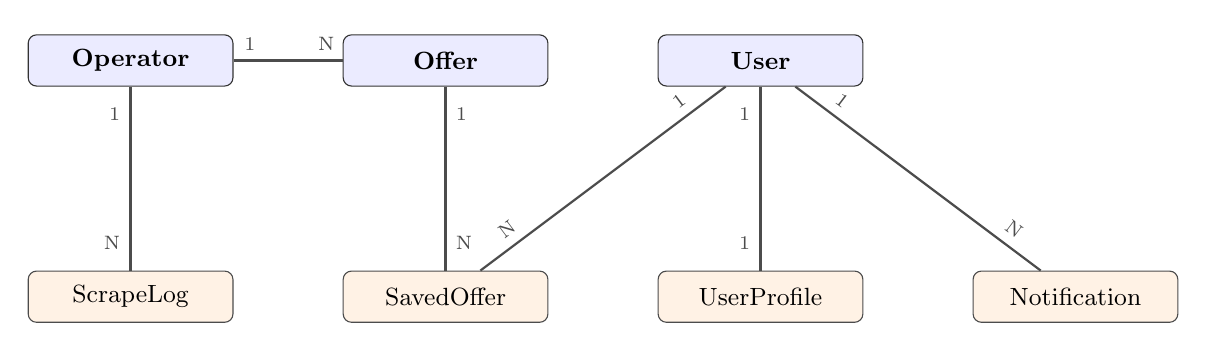
\begin{tikzpicture}[
  entity/.style={rectangle, draw=black!80, fill=blue!8, rounded corners=3pt,
                 minimum width=2.6cm, minimum height=0.65cm, align=center, font=\small\bfseries},
  assoc/.style={rectangle, draw=black!70, fill=orange!10, rounded corners=3pt,
                minimum width=2.6cm, minimum height=0.65cm, align=center, font=\small},
  line/.style={thick, black!70}
]
  % ── Row 1: Strong entities ─────────────────────────────────────────────
  \node[entity] (operator)  at ( 0,   0) {Operator};
  \node[entity] (offer)     at ( 4.0, 0) {Offer};
  \node[entity] (user)      at ( 8.0, 0) {User};

  % ── Row 2: Dependent entities ──────────────────────────────────────────
  \node[assoc]  (scrapelog) at ( 0,  -3) {ScrapeLog};
  \node[assoc]  (saved)     at ( 4.0,-3) {SavedOffer};
  \node[assoc]  (profile)   at ( 8.0,-3) {UserProfile};
  \node[assoc]  (notif)     at (12.0,-3) {Notification};

  % ── Relationships ──────────────────────────────────────────────────────
  % Operator → Offer  (1 : N)
  \draw[line] (operator) -- node[above, font=\scriptsize, pos=0.15]{1}
                             node[above, font=\scriptsize, pos=0.85]{N} (offer);
  % Operator → ScrapeLog  (1 : N)
  \draw[line] (operator) -- node[left, font=\scriptsize, pos=0.15]{1}
                             node[left, font=\scriptsize, pos=0.85]{N} (scrapelog);
  % Offer → SavedOffer  (1 : N)
  \draw[line] (offer)    -- node[right, font=\scriptsize, pos=0.15]{1}
                             node[right, font=\scriptsize, pos=0.85]{N} (saved);
  % User → SavedOffer  (1 : N, diagonal)
  \draw[line] (user)     -- node[above, sloped, font=\scriptsize, pos=0.15]{1}
                             node[above, sloped, font=\scriptsize, pos=0.85]{N} (saved);
  % User → UserProfile  (1 : 1)
  \draw[line] (user)     -- node[left, font=\scriptsize, pos=0.15]{1}
                             node[left, font=\scriptsize, pos=0.85]{1} (profile);
  % User → Notification  (1 : N, diagonal)
  \draw[line] (user)     -- node[above, sloped, font=\scriptsize, pos=0.15]{1}
                             node[above, sloped, font=\scriptsize, pos=0.85]{N} (notif);
\end{tikzpicture}
\caption{Entity-relationship diagram of the Mobile Match Algeria data model}
\label{fig:erd}
\end{figure}

\subsection{Prisma Schema Description}

The Prisma schema defines the relational structure. Table~\ref{tab:entities} summarises the key entities, their principal attributes, and their relationships.

\begin{table}[H]
  \caption{Key entities and their principal attributes}
  \label{tab:entities}
  \centering\small
  \begin{tabular}{|p{2.3cm}|p{8.0cm}|p{3.9cm}|}
    \hline
    \textbf{Entity}  & \textbf{Key attributes} & \textbf{Relationships} \\
    \hline
    Operator    & id, name, slug, logoUrl, primaryColor, websiteUrl & 1:N Offer; 1:N ScrapeLog \\
    \hline
    Offer       & id, name, slug, type, priceDA, dataGB, voiceMinutes, smsCount, validityDays, network, isActive & N:1 Operator; N:M User (via SavedOffer) \\
    \hline
    User        & id, name, email, passwordHash, role & 1:1 UserProfile; 1:N SavedOffer; 1:N Notification \\
    \hline
    UserProfile & id, monthlyBudget, dataUsageGB, voiceMinutes, smsCount, preferredType, preferredNet & 1:1 User \\
    \hline
    SavedOffer  & id, savedAt & N:1 User; N:1 Offer \\
    \hline
    Notification & id, title, message, isRead, createdAt & N:1 User \\
    \hline
    ScrapeLog   & id, operatorId, status, offersFound, offersAdded, offersUpdated, errorMessage, duration & N:1 Operator \\
    \hline
  \end{tabular}
\end{table}

\section{System Architecture}

\subsection{Three-Tier Architecture}

The application follows a classic three-tier architecture. The \textbf{presentation tier} consists of React components rendered by Next.js, either on the server (for initial page load) or on the client (for interactive elements). The \textbf{logic tier} consists of Next.js API route handlers located in the \texttt{src/app/api/} directory, which implement the business logic and data access layer. The \textbf{data tier} consists of a SQLite database accessed exclusively through Prisma.

Figure~\ref{fig:arch-overview} illustrates the high-level component architecture.

\begin{figure}[H]
\centering
\begin{tikzpicture}[
  tierbox/.style={rectangle, draw=black!60, rounded corners=5pt,
                  minimum width=14cm, minimum height=1.6cm, align=center},
  tierlabel/.style={rectangle, draw=black!60, rounded corners=3pt,
                    minimum width=2.8cm, minimum height=1.4cm, align=center,
                    font=\small\bfseries},
  comp/.style={rectangle, draw=black!45, fill=white, rounded corners=3pt,
               minimum width=3.5cm, minimum height=0.72cm, align=center, font=\scriptsize},
  biarrow/.style={{Stealth[length=5pt]}-{Stealth[length=5pt]}, thick, black!60}
]
  % ── Tier 1 — Presentation ──────────────────────────────────────────
  \node[tierbox,  fill=blue!6]   (box1) at (7.0, 4.0) {};
  \node[tierlabel, fill=blue!18, anchor=west]  at ([xshift=2mm]box1.west) {Presentation\\Tier};
  \node[comp, fill=blue!14] at (5.0, 4.0) {Offers Page};
  \node[comp, fill=blue!14] at (8.5, 4.0) {Compare Page};
  \node[comp, fill=blue!14] at (12.0, 4.0) {Admin Dashboard};

  % ── Tier 2 — Logic / API ───────────────────────────────────────────
  \node[tierbox,  fill=green!5]  (box2) at (7.0, 2.0) {};
  \node[tierlabel, fill=green!18, anchor=west] at ([xshift=2mm]box2.west) {Logic Tier\\(API)};
  \node[comp, fill=green!14] at (5.0, 2.0) {/api/offers};
  \node[comp, fill=green!14] at (8.5, 2.0) {/api/recommendations};
  \node[comp, fill=green!14] at (12.0, 2.0) {Scraper + Cron};

  % ── Tier 3 — Data ──────────────────────────────────────────────────
  \node[tierbox,  fill=orange!5] (box3) at (7.0, 0.0) {};
  \node[tierlabel, fill=orange!20, anchor=west] at ([xshift=2mm]box3.west) {Data Tier};
  \node[comp, fill=orange!14] at (5.0, 0.0) {Prisma ORM};
  \node[comp, fill=orange!14] at (8.5, 0.0) {SQLite Database};
  \node[comp, fill=orange!14] at (12.0, 0.0) {ScrapeLog};

  % ── Connecting arrows (one per gap, bidirectional) ─────────────────
  \draw[biarrow] (7.0, 3.2) -- node[right=2mm, font=\scriptsize]{HTTP requests / JSON responses} (7.0, 2.8);
  \draw[biarrow] (7.0, 1.2) -- node[right=2mm, font=\scriptsize]{Prisma queries / typed results}  (7.0, 0.8);
\end{tikzpicture}
\caption{High-level three-tier architecture of Mobile Match Algeria}
\label{fig:arch-overview}
\end{figure}

\subsection{API Route Map}

Table~\ref{tab:api-routes-design} lists the main API routes, their HTTP methods, and their functions.

\begin{table}[H]
  \caption{API route map (design overview)}
  \label{tab:api-routes-design}
  \centering\small
  \begin{tabular}{|p{4.2cm}|p{2.6cm}|p{7.0cm}|}
    \hline
    \textbf{Route} & \textbf{Method(s)} & \textbf{Function} \\
    \hline
    \texttt{/api/offers}          & GET                & List and filter offers; also serves by \texttt{ids} for comparison \\
    \hline
    \texttt{/api/offers/[id]}     & GET, PATCH, DELETE & Retrieve offer detail with similar offers; admin-only toggle of \texttt{isActive} (PATCH) or soft-delete (DELETE) \\
    \hline
    \texttt{/api/saved-offers}    & GET, POST          & List saved offer IDs; toggle save/unsave for authenticated user \\
    \hline
    \texttt{/api/recommendations} & POST               & Return top-3 scored plans for the submitted user profile \\
    \hline
    \texttt{/api/notifications}   & GET, PATCH, DELETE & List, mark-all-read, or delete a notification \\
    \hline
    \texttt{/api/profile}         & GET, PUT           & Retrieve or update the authenticated user's profile \\
    \hline
    \texttt{/api/admin/stats}      & GET                & Platform statistics (users, active offers, scrape sessions, operator health) \\
    \hline
    \texttt{/api/admin/scrape}     & POST               & Trigger a full scrape run across all three operators \\
    \hline
    \texttt{/api/stats}           & GET                & Public platform statistics (offer count, operator count) \\
    \hline
  \end{tabular}
\end{table}

\section{UI/UX Design}

\subsection{Design Principles}

The interface design of \textit{Mobile Match Algeria} is guided by five principles. First, \textbf{clarity}: information hierarchy is conveyed through typographic weight and spatial grouping rather than decorative elements, so users can locate the data they need at a glance. Second, \textbf{feedback}: every user action — saving a plan, comparing, triggering a scrape — produces an immediate visual response (toast notification, button state change, loading indicator). Third, \textbf{consistency}: the same card component, the same filter pills, and the same button styles appear throughout the application, reducing the cognitive load of navigation. Fourth, \textbf{responsiveness}: the interface reflows gracefully from 320~px mobile widths to wide desktop screens using CSS Grid and flexbox. Fifth, \textbf{accessibility}: interactive elements are keyboard-navigable and colour contrast ratios meet the WCAG~2.1 AA standard.

\subsection{Key Interface Screens}

The application comprises six main screens, whose appearance is illustrated by the screenshots embedded in Chapter~3, Section~3.5.

\begin{enumerate}
  \item \textbf{Home page} — Language-selection landing page presenting feature highlights (plan comparison, personalised recommendations, saved favourites, live data) and operator logos. Authenticated users are redirected directly to the offers page.
  \item \textbf{Offers page} — Grid of offer cards with operator filter tabs, plan type pills, and an advanced filter panel (price, data, network). A sticky bottom bar appears when plans are selected for comparison.
  \item \textbf{Comparison page} — Side-by-side table with row-level highlighting for the best value per attribute across price, data, voice, SMS, and validity.
  \item \textbf{Recommendations page} — Usage profile form (sliders for budget, data, voice, SMS; toggles for type and network) followed by a ranked list of matched plans with score explanations.
  \item \textbf{Login and Registration} — Authentication screens for account creation and sign-in, with client-side validation and inline error feedback.
  \item \textbf{Admin dashboard} — Four statistics cards (active offers, registered users, scrape sessions, scrape success rate), operator health panel with per-operator offer counts and last-scrape timestamps, detailed scrape history log, and a notifications tab for system and recommendation alerts.
\end{enumerate}

\section{Technology Stack Justification}

Table~\ref{tab:tech-choices} presents the technology choices made for this project alongside the main alternatives considered, with the rationale for each decision.

\begin{table}[H]
  \caption{Technology stack choices and justifications}
  \label{tab:tech-choices}
  \centering\small
  \begin{tabular}{|p{3.2cm}|p{2.3cm}|p{3.2cm}|p{5.0cm}|}
    \hline
    \textbf{Component}   & \textbf{Chosen}       & \textbf{Alternative}      & \textbf{Rationale} \\
    \hline
    Full-stack framework & Next.js 16            & Nuxt (Vue), SvelteKit     & Mature ecosystem, unified front/back codebase, strong TypeScript support \\
    \hline
    Language             & TypeScript            & JavaScript                & Compile-time type safety reduces runtime errors \\
    \hline
    ORM                  & Prisma                & TypeORM, raw SQL          & Auto-generated types, readable schema DSL, migration tooling \\
    \hline
    Database             & SQLite                & PostgreSQL, MySQL         & Zero-config deployment for single-server use; sufficient for current scale \\
    \hline
    Authentication       & NextAuth.js           & Passport.js, custom JWT   & Tight Next.js integration, built-in session management \\
    \hline
    Styling              & CSS custom properties & Tailwind CSS, CSS Modules & Fine-grained theming (dark mode), no build dependency \\
    \hline
    Animations           & Framer Motion         & React Spring, CSS only    & Declarative, performant, minimal boilerplate \\
    \hline
  \end{tabular}
\end{table}

\section*{Chapter Summary}

This chapter has formalised the functional and non-functional requirements of the system, identified the three actor types, modelled the key use cases and interaction flows through UML diagrams, defined the data model, described the three-tier architecture and API route map, articulated the UI/UX design principles, and justified the technology stack. The design decisions documented here form the blueprint for the implementation described in Chapter~3.
